\documentclass[mathserif,serif]{beamer}
\usepackage{tabularx}
\setbeamertemplate{footline}[frame number]
% \useoutertheme{infolines}
\usepackage{slidesphysics}
\graphicspath{{../plot/}}

\title[]{SS Analysis}
\author[]
{
Samuel Lo \inst{1}
\and
Yanjun Tu  \inst{1}
\and
Dongliang Zhang  \inst{2}
}
\institute[]
{
\inst{1}
The University of Hong Kong
\and
\inst{2}
University of Michigan
}
\date[]{\today}

\newcommand\Wider[2][3em]{%
\makebox[\linewidth][c]{%
\begin{minipage}{\dimexpr\textwidth+#1\relax}
\raggedright
\centering#2
\end{minipage}%
}%
}

\begin{document}
\frame{\titlepage}

\begin{frame}{Introduction}
\begin{itemize}
\item Update on the optimization
\begin{itemize}
\item Use Jeanette suggestion: The yields of groups of BG need to be positive.
\end{itemize}
\item Check the charge flip background
\begin{itemize}
\item Compare data and MC background
\item Compare data and data-driven background (estimation from data OS events)
\end{itemize}
\end{itemize}
\end{frame}

\begin{frame}
\begin{center}
\huge
Update on the optimization
\end{center}
\end{frame}

\begin{frame}{optimization constraints}
\small
The following constraints are applied to reduce the bias from low statistics:
\begin{itemize}
\small
\item The yields of groups of BG need to be positive, except multi-top, V+gamma and Z+jets.
\begin{itemize}
\item To have a reasonable/stable modeling of the background shape.
\item In practice, the HistFitter will include the background only when it has positive yield.
\end{itemize}
\item At least 10 unweighted events in VV and ttV background.
\item If the yield for one group of BG is negative, 0 yield is used. But the statistical error still keep unchanged to calculate the statistical error of total BG.
\item nSig$>$1 and nSig/nSigError $>$ 2 for both (162.5,12.5) and (175,0).
\item For $\pt^{l1}$, $\pt^{l1}$, $\pt^{ll}$, $m_{T2}$, $E_{\text{T}}^{\text{miss,rel}}$, $m_{\text{eff}}$ and $m_{\text{T}}^{\text{max}}$, there is no upper cut.
\item For $|\Delta\eta_{ll}|$ and $m_{lj}$/$m_{ljj}$, there is no lower cut.
\end{itemize}
\end{frame}

\begin{frame}{Cuts in SR}
\vspace{5mm}
\tiny
\begin{tabular}{|c|c|c|c|c|c|c|}
\hline
& SR$ee$-1 & SR$ee$-2 & SR$\mu\mu$-1 & SR$\mu\mu$-2 & SR$e\mu$-1 & SR$e\mu$-2 \\
\hline
Lepton flavours & $ee$ & $ee$ & $\mu\mu$ & $\mu\mu$ & $e\mu$ & $e\mu$ \\
\hline
$n_{cjets}$ & 1 & 2 or 3 & 1 & 2 or 3 & 1 & 2 or 3 \\
\hline
\begin{tabular}{|c|c|c|c|c|c|c|}
\hline
& SR$ee$-1 & SR$ee$-2 & SR$\mu\mu$-1 & SR$\mu\mu$-2 & SR$e\mu$-1 & SR$e\mu$-2 \\
\hline
Lepton flavours & $ee$ & $ee$ & $\mu\mu$ & $\mu\mu$ & $e\mu$ & $e\mu$ \\
\hline
$n_{cjets}$ & 1 & 2 or 3 & 1 & 2 or 3 & 1 & 2 or 3 \\
\hline
Leading lepton \pt [GeV] & $\geq 65$ & $\geq 25$ & $\geq 25$ & $\geq 25$ & $\geq 25$ & $\geq 25$ \\
\hline
Sub-leading lepton \pt [GeV] & $\geq 25$ & $\geq 25$ & $\geq 25$ & $\geq 25$ & $\geq 25$ & $\geq 25$ \\
\hline
$|m_{ll}-m_Z|$ [GeV] & $>10$ & $>10$ & - & - & - & - \\
\hline
$|\Delta\eta_{ll}|$ & $<1.5$ & $<1.5$ & $<1.5$ & $<1.5$ & $<1.5$ & $<1.5$ \\
\hline
$E_{\text{T}}^{\text{miss,rel}}$ [GeV] & - & $\geq 65$ & - & $\geq 40$ & $\geq 80$ & $\geq 25$ \\
\hline
$m_{\text{eff}}$ [GeV] & $\geq 200$ & $\geq 200$ & $\geq 200$ & $\geq 200$ & $\geq 200$ & $\geq 200$ \\
\hline
$m_{\text{T}}^{\text{max}}$ [GeV] & $\geq 125$ & $\geq 85$ & $\geq 100$ & $\geq 75$ & - & $\geq 105$ \\
\hline
$m_{lj}$/$m_{ljj}$ [GeV] & $<105$ & $<205$ & $<100$ & $<160$ & $<95$ & $<255$ \\
\hline
$m_{T2}$ [GeV] & - & $\geq 15$ & - & - & - & $\geq 75$ \\
\hline
$\pt^{ll}$ [GeV] & - & - & - & $\geq 40$ & - & - \\
\hline

\end{tabular}
\end{frame}

\begin{frame}{Yields and significance in SR}
\includegraphics[width=\textwidth]{SR_SS_opt}
\end{frame}

\begin{frame}{signal yield plot}
\Wider[5em]{
\includegraphics[width=0.33\textwidth]{nSig_SR_SS_ee_1_opt_0}
\includegraphics[width=0.33\textwidth]{nSig_SR_SS_mumu_1_opt_0}
\includegraphics[width=0.33\textwidth]{nSig_SR_SS_emu_1_opt_0} \\
\includegraphics[width=0.33\textwidth]{nSig_SR_SS_ee_2_opt_0}
\includegraphics[width=0.33\textwidth]{nSig_SR_SS_mumu_2_opt_0}
\includegraphics[width=0.33\textwidth]{nSig_SR_SS_emu_2_opt_0}
}
\end{frame}

\begin{frame}{significance plot}
\Wider{
\includegraphics[width=0.33\textwidth]{significance_SR_SS_ee_1_opt_0}
\includegraphics[width=0.33\textwidth]{significance_SR_SS_mumu_1_opt_0}
\includegraphics[width=0.33\textwidth]{significance_SR_SS_emu_1_opt_0} \\
\includegraphics[width=0.33\textwidth]{significance_SR_SS_ee_2_opt_0}
\includegraphics[width=0.33\textwidth]{significance_SR_SS_mumu_2_opt_0}
\includegraphics[width=0.33\textwidth]{significance_SR_SS_emu_2_opt_0}
}
\end{frame}


\begin{frame}{Compare with the old one}
\begin{itemize}
\item Combine the significance (only channels with $Z_n>0$ are combined)
\end{itemize}
\includegraphics[width=0.5\textwidth]{data/optimization/old_opt}
\includegraphics[width=0.5\textwidth]{data/optimization/new_opt}
\end{frame}

\begin{frame}
\begin{center}
\huge
Check the charge flip background
\end{center}
\end{frame}

\begin{frame}{SS\_ee Control Region}
\begin{itemize}
\item Define SS\_ee Control Region:
\begin{itemize}
\item $|m_{ll}-m_Z| < 10$ GeV
\end{itemize}
\item The $m_{ll}$ plot is a N-1 plot.
\end{itemize}
\end{frame}

\begin{frame}
\begin{center}
\huge
Compare data and MC background
\end{center}
\end{frame}

\input{data/expN_CR_SS_ee_Zmass_MC.tex}
\input{data/plot_CR_SS_ee_Zmass_MC.tex}

\begin{frame}
\begin{center}
\huge
Compare data and data-driven background \\
\normalsize
(estimation from data OS events) \\
replace Z+jets, ttbar and Wt
\end{center}
\end{frame}

\input{data/expN_CR_SS_ee_Zmass_data.tex}
\input{data/plot_CR_SS_ee_Zmass_data.tex}

\section{Conclusion}
\begin{frame}{Conclusion}
\begin{itemize}
\item About the two optimizations, which one is better/prefered?
\item Charge flip background
\begin{itemize}
\item Overestimation in MC
\item $\pt$ shift in data-driven BG (need to check with Gabriel)
\end{itemize}
\end{itemize}
\end{frame}

\section{Plan}
\begin{frame}{Plan}
\begin{itemize}
\item Optimization with data-driven charge flip background
\item Try different trigger combination
\item Try different $\eta$ cut for baseline muons
\item Try different $\eta$ cut for jets
\end{itemize}
\end{frame}

\begin{frame}
\begin{center}
\huge
Backup
\end{center}
\end{frame}

\begin{frame}
\small
SUSY scenario:\\
\begin{figure}
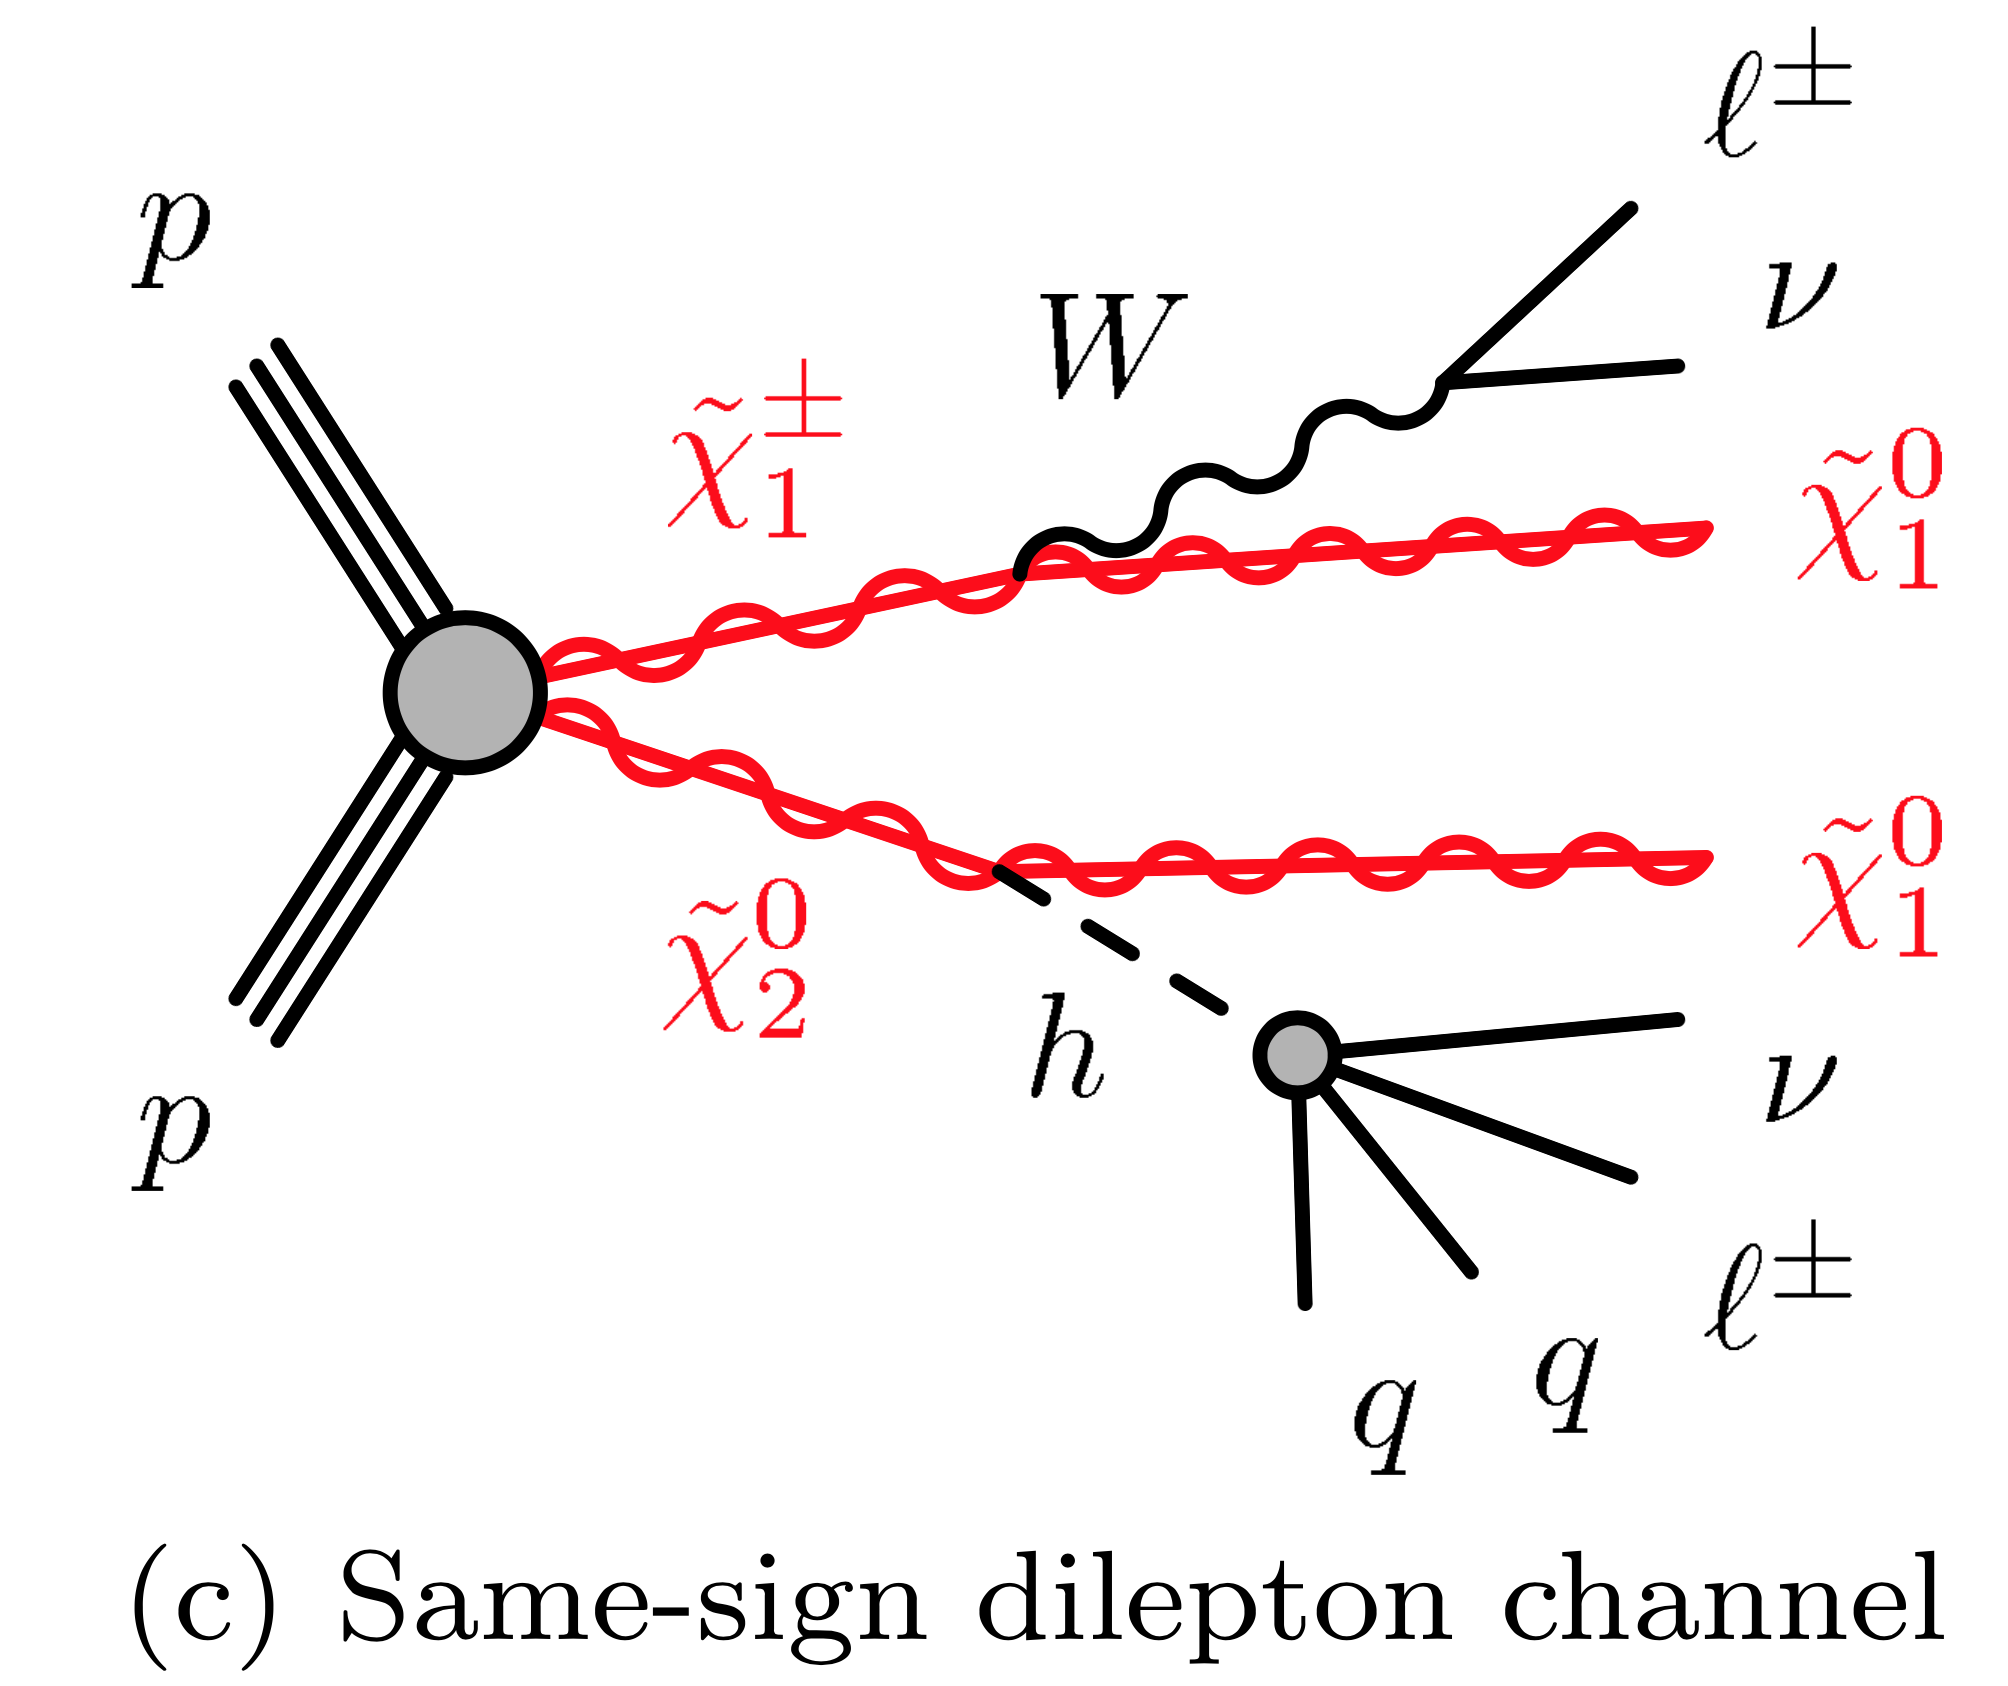
\includegraphics[width=0.6\textwidth]{data/photo/Wh.png}
\end{figure}
\end{frame}

\begin{frame}[fragile]
\frametitle{Signal sample}
\small
Sample Name(p2949 tag):
\tiny
\begin{verbatim}
mc15_13TeV.
393822.MGPy8EG_A14N23LO_C1N2_Wh_hall_162p5_12p5_2L7.merge.DAOD_SUSY2.e6153_a766_a821_r7676_p2949

mc15_13TeV.
393823.MGPy8EG_A14N23LO_C1N2_Wh_hall_175p0_0p0_2L7.merge.DAOD_SUSY2.e6153_a766_a821_r7676_p2949

mc15_13TeV.
393895.MGPy8EG_A14N23LO_C1N2_Wh_hall_450p0_0p0_2L7.merge.DAOD_SUSY2.e6153_a766_a821_r7676_p2949
\end{verbatim}
\end{frame}

\begin{frame}[fragile]
\frametitle{Data}
\small
use both 2015 and 2016 data (3212.96 + 32861.6) /pb
\tiny
\begin{verbatim}
GRL:
GoodRunsLists/data16_13TeV/20161101/physics_25ns_20.7.xml
GoodRunsLists/data15_13TeV/20160720/physics_25ns_20.7.xml
\end{verbatim}
\end{frame}

\begin{frame}{MC BG}
p-tag: p2949
\end{frame}

\begin{frame}[fragile]
\small
Trigger list:\\
\scriptsize
\begin{verbatim}
2015
HLT_2e12_lhloose_L12EM10VH
HLT_e17_lhloose_mu14
HLT_mu18_mu8noL1

2016(A-D3)
HLT_2e17_lhvloose_nod0
HLT_e17_lhloose_nod0_mu14
HLT_mu20_mu8noL1

2016(D3-)
HLT_2e17_lhvloose_nod0
HLT_e17_lhloose_nod0_mu14
HLT_mu22_mu8noL1
\end{verbatim}
\end{frame}

\begin{frame}{Object Definitions}
\small
Tool: AnalysisBase 2.4.31, SUSYTools-00-08-60\\

\centering
\begin{table}
\small
\begin{tabularx}{\textwidth}{p{1.5cm} | p{3cm} | p{3cm} | p{3cm}}
& \textbf{Electron} & \textbf{Muon} & \textbf{Jet}\\
\hline
\textbf{Baseline}
& - $p_T>10$ GeV \newline - $|\eta^{cluster}| < 2.47$ \newline - LooseAndBLayerLLH
& - $p_T>10$ GeV \newline - $|\eta| < 2.4$ \newline - Medium
& - $p_T>20$ GeV \\
\hline
\textbf{Signal}
& - $p_T > 20$ GeV \newline - $|\eta^{cluster}| < 2.47$ \newline - MediumLLH \newline - FixedCutTight \newline - $|z_0 \sin \theta| < 0.5$mm \newline - $|d_0/\sigma_{d_0}| < 5$
& - $p_T > 20$ GeV \newline - $|\eta| < 2.4$ \newline - Medium \newline - GradientLoose \newline - $|z_0 \sin \theta| < 0.5$mm \newline - $|d_0/\sigma_{d_0}| < 3$
& - $p_T > 20$ GeV \newline - $|\eta|<2.8$ \newline \newline - $|JVT| > 0.59$ \newline if $p_T < 60$ GeV \newline and $|\eta| < 2.4$
\end{tabularx}
\end{table}

\raggedright
Selection:
\begin{itemize}
\item Trigger requirement
\item Exactly 2 baseline leptons and exactly 2 signal leptons
\end{itemize}

\tiny
Note: \\
Pileup reweighting is applied. \\
Scale factor for reconstruction, isolation, ID and trigger is applied.
\end{frame}

%\begin{frame}
%\frametitle{averageMu}
%\begin{figure}
%\includegraphics[width=0.33\textwidth]{averageMu_CR_ISR_OS_ee}
%\includegraphics[width=0.33\textwidth]{averageMu_CR_ISR_OS_mumu}
%\includegraphics[width=0.33\textwidth]{averageMu_CR_ISR_OS_emu} \\
%\caption{Average number of interactions per bunch crossing, for ee channel (left), $\mu\mu$ channel (middle) and e$\mu$ channel (right).}
%\end{figure}
%\end{frame}

\begin{frame}
\frametitle{Definition of jets}
\normalsize
\begin{itemize}
\item Central jets: $\pt>20$ GeV, $|\eta|<2.8$, no b-tagged
\begin{itemize}
\item Use new eta cut.
\end{itemize}
\item B-jets: b-tagged
\end{itemize}
\end{frame}

\begin{frame}
\frametitle{significance calculation}
\begin{itemize}
\item RooStats::NumberCountingUtils::BinomialExpZ(S,B,$\delta$B)
\item $\delta$B = sqrt((0.25)\^{}2 + (nBGError/nBG)\^{}2)
\begin{itemize}
\item use the same definition from Dani.
\end{itemize}
\end{itemize}
\end{frame}

\begin{frame}
\frametitle{definition of variables}
\normalsize
\begin{itemize}
\item HT: Sum of the $p_T$ of all signal jets and the two leptons.
\item R2 = MET / (MET + pt1 + pt2)
\item l12\_dPhi: difference in phi between the two leptons.
\item l12\_MET\_dPhi: difference in phi between MET and the sum of 4-momentum of the two leptons.
\end{itemize}
\end{frame}

\begin{frame}{Selection in run1 SR}
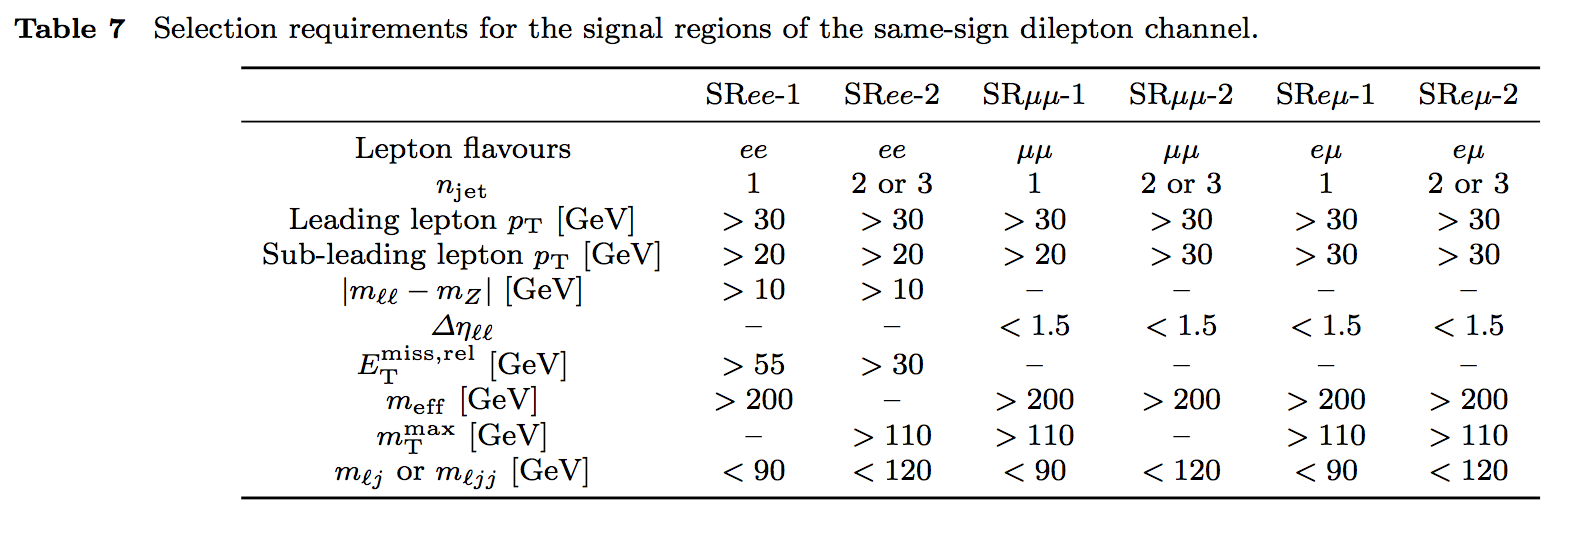
\includegraphics[width=\textwidth]{data/photo/SRcutrun1.png} \\
\url{https://arxiv.org/pdf/1501.07110.pdf}
\end{frame}

\begin{frame}
\begin{center}
\huge
Pre-selection plot
\end{center}
\end{frame}

\begin{frame}{Pre-selection cut}
\normalsize
\begin{columns}
\begin{column}{0.5\textwidth}

\begin{itemize}
\item SR$ee$1
\begin{itemize}
\item nCJet $=1$
\item nBJet $=0$
\item $|m_{ll} - 91.2| > 10$
\end{itemize}
\item SR$\mu\mu$1
\begin{itemize}
\item nCJet $=1$
\item nBJet $=0$
\end{itemize}
\item SR$e\mu$1
\begin{itemize}
\item nCJet $=1$
\item nBJet $=0$
\end{itemize}
\end{itemize}

\end{column}
\begin{column}{0.5\textwidth}

\begin{itemize}
\item SR$ee$2
\begin{itemize}
\item nCJet $=2$ or $3$
\item nBJet $=0$
\item $|m_{ll} - 91.2| > 10$
\end{itemize}
\item SR$\mu\mu$2
\begin{itemize}
\item nCJet $=2$ or $3$
\item nBJet $=0$
\end{itemize}
\item SR$e\mu$2
\begin{itemize}
\item nCJet $=2$ or $3$
\item nBJet $=0$
\end{itemize}
\end{itemize}

\end{column}
\end{columns}
\end{frame}

\begin{frame}{Expected number of events \\ For SR\_SS\_ee\_1\_pre}
\vspace{5mm}
\begin{tabular}{|c|c|c|}
\hline
& Number of events & Significance \\
\hline
Z+jets & $1041.127228\pm153.507203$ (1003) & \\
\hline
W+jets & $255.071259\pm85.080870$ (223) & \\
\hline
V$+\gamma$ & $242.385849\pm13.376917$ (768) & \\
\hline
VV & $217.914223\pm5.009122$ (28876) & \\
\hline
$t\bar{t}$ & $11.460234\pm3.301990$ (25) & \\
\hline
Higgs & $9.826902\pm2.298310$ (105) & \\
\hline
single top & $5.452925\pm1.307231$ (29) & \\
\hline
VVV & $2.095896\pm0.165902$ (325) & \\
\hline
$t\bar{t}+V$ & $0.391007\pm0.058742$ (137) & \\
\hline
multi top & $0.000000\pm0.000000$ (0) & \\
\hline
Total BG & $1785.725523\pm176.139644$ (31491) & \\
\hline
(162.5,12.5) & $23.53\pm1.71$ (224) &$-0.13$\\
\hline
(202.5,72.5) & $8.98\pm1.16$ (76) &$-0.16$\\
\hline
(450.0,0.0) & $0.29\pm0.11$ (8) &$-0.18$\\
\hline

\end{tabular}
\end{frame}

\begin{frame}{Expected number of events \\ For SR\_SS\_mumu\_1\_pre}
\vspace{5mm}
\begin{tabular}{|c|c|c|}
\hline
& Number of events & Significance \\
\hline
Z+jets & $-0.903811\pm6.921583$ (71) & \\
\hline
W+jets & $70.328256\pm21.240156$ (172) & \\
\hline
$t\bar{t}$ & $7.686362\pm1.562601$ (26) & \\
\hline
single top & $4.829827\pm1.162325$ (27) & \\
\hline
$t\bar{t}+V$ & $0.642968\pm0.065700$ (219) & \\
\hline
multi top & $0.000000\pm0.000000$ (0) & \\
\hline
VV & $273.201006\pm4.447218$ (39240) & \\
\hline
V$+\gamma$ & $0.000000\pm0.000000$ (0) & \\
\hline
VVV & $3.239846\pm0.204705$ (558) & \\
\hline
Higgs & $13.056766\pm2.332374$ (53) & \\
\hline
Total BG & $372.985031\pm22.980626$ (40366) & \\
\hline
(162.5,12.5) & $37.34\pm2.30$ (333) &$0.20$\\
\hline
(202.5,72.5) & $15.99\pm1.63$ (124) &$-0.01$\\
\hline
(450.0,0.0) & $0.58\pm0.18$ (14) &$-0.17$\\
\hline

\end{tabular}
\end{frame}

\begin{frame}{Expected number of events \\ For SR\_SS\_emu\_1\_pre}
\vspace{5mm}
\begin{tabular}{|c|c|c|}
\hline
& Number of events & Significance \\
\hline
Z+jets & $93.750413\pm40.567822$ (255) & \\
\hline
W+jets & $324.962656\pm118.077523$ (461) & \\
\hline
$t\bar{t}$ & $20.441992\pm4.040177$ (50) & \\
\hline
single top & $7.393506\pm1.488672$ (39) & \\
\hline
$t\bar{t}+V$ & $0.864343\pm0.107271$ (318) & \\
\hline
multi top & $0.000000\pm0.000000$ (0) & \\
\hline
VV & $447.990089\pm5.885438$ (64261) & \\
\hline
V$+\gamma$ & $209.621932\pm12.089898$ (654) & \\
\hline
VVV & $5.195837\pm0.279168$ (832) & \\
\hline
Higgs & $14.832354\pm2.588111$ (111) & \\
\hline
Total BG & $1125.053123\pm125.674900$ (66981) & \\
\hline
Signal (175, 0) & $107.21\pm5.96$ (421) &$0.16$\\
\hline
Signal (165, 35) & $139.59\pm7.59$ (434) &$0.26$\\
\hline
Signal (400, 0) & $5.24\pm0.29$ (422) &$-0.16$\\
\hline

\end{tabular}
\end{frame}

\begin{frame}{Expected number of events \\ For SR\_SS\_ee\_2\_pre}
\vspace{5mm}
\begin{tabular}{|c|c|c|}
\hline
& Number of events & Significance \\
\hline
Z+jets & $551.366032\pm136.406644$ (2003) & \\
\hline
W+jets & $270.640170\pm89.121489$ (490) & \\
\hline
$t\bar{t}$ & $37.735436\pm4.464428$ (110) & \\
\hline
single top & $3.497454\pm0.911242$ (22) & \\
\hline
$t\bar{t}+V$ & $3.491800\pm0.161654$ (1398) & \\
\hline
multi top & $0.002190\pm0.001936$ (2) & \\
\hline
VV & $277.387999\pm4.692851$ (67416) & \\
\hline
V$+\gamma$ & $203.651192\pm12.534853$ (813) & \\
\hline
VVV & $2.297767\pm0.181863$ (480) & \\
\hline
Higgs & $15.839962\pm3.076694$ (218) & \\
\hline
Total BG & $1365.910003\pm163.581309$ (72952) & \\
\hline
Signal (175, 0) & $48.30\pm3.78$ (188) &$-0.06$\\
\hline
Signal (165, 35) & $66.77\pm5.81$ (201) &$-0.01$\\
\hline
Signal (400, 0) & $4.14\pm0.31$ (323) &$-0.17$\\
\hline

\end{tabular}
\end{frame}

\begin{frame}{Expected number of events \\ For SR\_SS\_mumu\_2\_pre}
\vspace{5mm}
\begin{tabular}{|c|c|c|}
\hline
& Number of events & Significance \\
\hline
Z+jets & $30.911743\pm16.623014$ (118) & \\
\hline
W+jets & $75.577828\pm16.297410$ (307) & \\
\hline
$t\bar{t}$ & $52.409081\pm4.246995$ (182) & \\
\hline
single top & $6.337801\pm1.795583$ (32) & \\
\hline
$t\bar{t}+V$ & $4.906009\pm0.187888$ (1921) & \\
\hline
multi top & $0.000238\pm0.000238$ (1) & \\
\hline
VV & $326.965631\pm4.030877$ (85579) & \\
\hline
V$+\gamma$ & $0.015268\pm0.010936$ (2) & \\
\hline
VVV & $3.488119\pm0.228909$ (632) & \\
\hline
Higgs & $20.014418\pm4.481653$ (196) & \\
\hline
Total BG & $520.626134\pm24.486982$ (88970) & \\
\hline
Signal (175, 0) & $103.17\pm6.73$ (353) &$0.56$\\
\hline
Signal (165, 35) & $112.31\pm6.52$ (364) &$0.62$\\
\hline
Signal (400, 0) & $4.87\pm0.26$ (407) &$-0.13$\\
\hline

\end{tabular}
\end{frame}

\begin{frame}{Expected number of events \\ For SR\_SS\_emu\_2\_pre}
\vspace{5mm}
\begin{tabular}{|c|c|c|}
\hline
& Number of events & Significance \\
\hline
Z+jets & $116.969752\pm23.521205$ (489) & \\
\hline
W+jets & $192.186476\pm76.464783$ (696) & \\
\hline
$t\bar{t}$ & $75.588083\pm5.272688$ (256) & \\
\hline
single top & $8.870611\pm1.460928$ (61) & \\
\hline
$t\bar{t}+V$ & $7.747451\pm0.250025$ (3158) & \\
\hline
multi top & $0.000873\pm0.000438$ (4) & \\
\hline
VV & $549.830395\pm4.903205$ (142285) & \\
\hline
V$+\gamma$ & $177.947444\pm13.158731$ (690) & \\
\hline
VVV & $5.524547\pm0.279397$ (1080) & \\
\hline
Higgs & $27.387550\pm3.643723$ (397) & \\
\hline
Total BG & $1162.053181\pm81.490224$ (149116) & \\
\hline
(162.5,12.5) & $68.66\pm3.10$ (646) &$0.05$\\
\hline
(202.5,72.5) & $36.08\pm2.61$ (281) &$-0.05$\\
\hline
(450.0,0.0) & $1.47\pm0.22$ (46) &$-0.17$\\
\hline

\end{tabular}
\end{frame}


\begin{frame}{For SR\_SS\_pre \\ $\pt^{l1}$}
\Wider[5em]{
\includegraphics[width=0.33\textwidth]{pt1_SR_SS_ee_1_pre}
\includegraphics[width=0.33\textwidth]{pt1_SR_SS_mumu_1_pre}
\includegraphics[width=0.33\textwidth]{pt1_SR_SS_emu_1_pre} \\
\includegraphics[width=0.33\textwidth]{pt1_SR_SS_ee_2_pre}
\includegraphics[width=0.33\textwidth]{pt1_SR_SS_mumu_2_pre}
\includegraphics[width=0.33\textwidth]{pt1_SR_SS_emu_2_pre}
}
\end{frame}

\begin{frame}{For SR\_SS\_pre \\ $\pt^{l2}$}
\Wider[5em]{
\includegraphics[width=0.33\textwidth]{pt2_SR_SS_ee_1_pre}
\includegraphics[width=0.33\textwidth]{pt2_SR_SS_mumu_1_pre}
\includegraphics[width=0.33\textwidth]{pt2_SR_SS_emu_1_pre} \\
\includegraphics[width=0.33\textwidth]{pt2_SR_SS_ee_2_pre}
\includegraphics[width=0.33\textwidth]{pt2_SR_SS_mumu_2_pre}
\includegraphics[width=0.33\textwidth]{pt2_SR_SS_emu_2_pre}
}
\end{frame}

\begin{frame}{For SR\_SS\_pre \\ $\eta^{l1}$}
\Wider[5em]{
\includegraphics[width=0.33\textwidth]{eta1_SR_SS_ee_1_pre}
\includegraphics[width=0.33\textwidth]{eta1_SR_SS_mumu_1_pre}
\includegraphics[width=0.33\textwidth]{eta1_SR_SS_emu_1_pre} \\
\includegraphics[width=0.33\textwidth]{eta1_SR_SS_ee_2_pre}
\includegraphics[width=0.33\textwidth]{eta1_SR_SS_mumu_2_pre}
\includegraphics[width=0.33\textwidth]{eta1_SR_SS_emu_2_pre}
}
\end{frame}

\begin{frame}{For SR\_SS\_pre \\ $\eta^{l2}$}
\Wider[5em]{
\includegraphics[width=0.33\textwidth]{eta2_SR_SS_ee_1_pre}
\includegraphics[width=0.33\textwidth]{eta2_SR_SS_mumu_1_pre}
\includegraphics[width=0.33\textwidth]{eta2_SR_SS_emu_1_pre} \\
\includegraphics[width=0.33\textwidth]{eta2_SR_SS_ee_2_pre}
\includegraphics[width=0.33\textwidth]{eta2_SR_SS_mumu_2_pre}
\includegraphics[width=0.33\textwidth]{eta2_SR_SS_emu_2_pre}
}
\end{frame}

\begin{frame}{For SR\_SS\_pre \\ $\phi^{l1}$}
\Wider[5em]{
\includegraphics[width=0.33\textwidth]{phi1_SR_SS_ee_1_pre}
\includegraphics[width=0.33\textwidth]{phi1_SR_SS_mumu_1_pre}
\includegraphics[width=0.33\textwidth]{phi1_SR_SS_emu_1_pre} \\
\includegraphics[width=0.33\textwidth]{phi1_SR_SS_ee_2_pre}
\includegraphics[width=0.33\textwidth]{phi1_SR_SS_mumu_2_pre}
\includegraphics[width=0.33\textwidth]{phi1_SR_SS_emu_2_pre}
}
\end{frame}

\begin{frame}{For SR\_SS\_pre \\ $m_{ll}$}
\Wider[5em]{
\includegraphics[width=0.33\textwidth]{mll_SR_SS_ee_1_pre}
\includegraphics[width=0.33\textwidth]{mll_SR_SS_mumu_1_pre}
\includegraphics[width=0.33\textwidth]{mll_SR_SS_emu_1_pre} \\
\includegraphics[width=0.33\textwidth]{mll_SR_SS_ee_2_pre}
\includegraphics[width=0.33\textwidth]{mll_SR_SS_mumu_2_pre}
\includegraphics[width=0.33\textwidth]{mll_SR_SS_emu_2_pre}
}
\end{frame}

\begin{frame}{For SR\_SS\_pre \\ $\pt^{ll}$}
\Wider[5em]{
\includegraphics[width=0.33\textwidth]{ptll_SR_SS_ee_1_pre}
\includegraphics[width=0.33\textwidth]{ptll_SR_SS_mumu_1_pre}
\includegraphics[width=0.33\textwidth]{ptll_SR_SS_emu_1_pre} \\
\includegraphics[width=0.33\textwidth]{ptll_SR_SS_ee_2_pre}
\includegraphics[width=0.33\textwidth]{ptll_SR_SS_mumu_2_pre}
\includegraphics[width=0.33\textwidth]{ptll_SR_SS_emu_2_pre}
}
\end{frame}

\begin{frame}{For SR\_SS\_pre \\ $E_{\text{T}}^{\text{miss}}$}
\Wider[5em]{
\includegraphics[width=0.33\textwidth]{MET_SR_SS_ee_1_pre}
\includegraphics[width=0.33\textwidth]{MET_SR_SS_mumu_1_pre}
\includegraphics[width=0.33\textwidth]{MET_SR_SS_emu_1_pre} \\
\includegraphics[width=0.33\textwidth]{MET_SR_SS_ee_2_pre}
\includegraphics[width=0.33\textwidth]{MET_SR_SS_mumu_2_pre}
\includegraphics[width=0.33\textwidth]{MET_SR_SS_emu_2_pre}
}
\end{frame}

\begin{frame}{For SR\_SS\_pre \\ $m_{T2}$}
\Wider[5em]{
\includegraphics[width=0.33\textwidth]{mTtwo_SR_SS_ee_1_pre}
\includegraphics[width=0.33\textwidth]{mTtwo_SR_SS_mumu_1_pre}
\includegraphics[width=0.33\textwidth]{mTtwo_SR_SS_emu_1_pre} \\
\includegraphics[width=0.33\textwidth]{mTtwo_SR_SS_ee_2_pre}
\includegraphics[width=0.33\textwidth]{mTtwo_SR_SS_mumu_2_pre}
\includegraphics[width=0.33\textwidth]{mTtwo_SR_SS_emu_2_pre}
}
\end{frame}

\begin{frame}{For SR\_SS\_pre \\ $m_{\text{T}}^{l1}$}
\Wider[5em]{
\includegraphics[width=0.33\textwidth]{mt1_SR_SS_ee_1_pre}
\includegraphics[width=0.33\textwidth]{mt1_SR_SS_mumu_1_pre}
\includegraphics[width=0.33\textwidth]{mt1_SR_SS_emu_1_pre} \\
\includegraphics[width=0.33\textwidth]{mt1_SR_SS_ee_2_pre}
\includegraphics[width=0.33\textwidth]{mt1_SR_SS_mumu_2_pre}
\includegraphics[width=0.33\textwidth]{mt1_SR_SS_emu_2_pre}
}
\end{frame}

\begin{frame}{For SR\_SS\_pre \\ $m_{\text{T}}^{l2}$}
\Wider[5em]{
\includegraphics[width=0.33\textwidth]{mt2_SR_SS_ee_1_pre}
\includegraphics[width=0.33\textwidth]{mt2_SR_SS_mumu_1_pre}
\includegraphics[width=0.33\textwidth]{mt2_SR_SS_emu_1_pre} \\
\includegraphics[width=0.33\textwidth]{mt2_SR_SS_ee_2_pre}
\includegraphics[width=0.33\textwidth]{mt2_SR_SS_mumu_2_pre}
\includegraphics[width=0.33\textwidth]{mt2_SR_SS_emu_2_pre}
}
\end{frame}

\begin{frame}{For SR\_SS\_pre \\ $\pt$ of the leading jet}
\Wider[5em]{
\includegraphics[width=0.33\textwidth]{jetpt_SR_SS_ee_1_pre}
\includegraphics[width=0.33\textwidth]{jetpt_SR_SS_mumu_1_pre}
\includegraphics[width=0.33\textwidth]{jetpt_SR_SS_emu_1_pre} \\
\includegraphics[width=0.33\textwidth]{jetpt_SR_SS_ee_2_pre}
\includegraphics[width=0.33\textwidth]{jetpt_SR_SS_mumu_2_pre}
\includegraphics[width=0.33\textwidth]{jetpt_SR_SS_emu_2_pre}
}
\end{frame}

\begin{frame}{For SR\_SS\_pre \\ $\eta$ of the leading jet}
\Wider[5em]{
\includegraphics[width=0.33\textwidth]{jeteta_SR_SS_ee_1_pre}
\includegraphics[width=0.33\textwidth]{jeteta_SR_SS_mumu_1_pre}
\includegraphics[width=0.33\textwidth]{jeteta_SR_SS_emu_1_pre} \\
\includegraphics[width=0.33\textwidth]{jeteta_SR_SS_ee_2_pre}
\includegraphics[width=0.33\textwidth]{jeteta_SR_SS_mumu_2_pre}
\includegraphics[width=0.33\textwidth]{jeteta_SR_SS_emu_2_pre}
}
\end{frame}

\begin{frame}{For SR\_SS\_pre \\ Number of jets}
\Wider[5em]{
\includegraphics[width=0.33\textwidth]{nJet_SR_SS_ee_1_pre}
\includegraphics[width=0.33\textwidth]{nJet_SR_SS_mumu_1_pre}
\includegraphics[width=0.33\textwidth]{nJet_SR_SS_emu_1_pre} \\
\includegraphics[width=0.33\textwidth]{nJet_SR_SS_ee_2_pre}
\includegraphics[width=0.33\textwidth]{nJet_SR_SS_mumu_2_pre}
\includegraphics[width=0.33\textwidth]{nJet_SR_SS_emu_2_pre}
}
\end{frame}

\begin{frame}{For SR\_SS\_pre \\ Number of b-jets}
\Wider[5em]{
\includegraphics[width=0.33\textwidth]{nBJet_SR_SS_ee_1_pre}
\includegraphics[width=0.33\textwidth]{nBJet_SR_SS_mumu_1_pre}
\includegraphics[width=0.33\textwidth]{nBJet_SR_SS_emu_1_pre} \\
\includegraphics[width=0.33\textwidth]{nBJet_SR_SS_ee_2_pre}
\includegraphics[width=0.33\textwidth]{nBJet_SR_SS_mumu_2_pre}
\includegraphics[width=0.33\textwidth]{nBJet_SR_SS_emu_2_pre}
}
\end{frame}

\begin{frame}{For SR\_SS\_pre \\ Number of central jets}
\Wider[5em]{
\includegraphics[width=0.33\textwidth]{nCJet_SR_SS_ee_1_pre}
\includegraphics[width=0.33\textwidth]{nCJet_SR_SS_mumu_1_pre}
\includegraphics[width=0.33\textwidth]{nCJet_SR_SS_emu_1_pre} \\
\includegraphics[width=0.33\textwidth]{nCJet_SR_SS_ee_2_pre}
\includegraphics[width=0.33\textwidth]{nCJet_SR_SS_mumu_2_pre}
\includegraphics[width=0.33\textwidth]{nCJet_SR_SS_emu_2_pre}
}
\end{frame}

\begin{frame}{For SR\_SS\_pre \\ $|\Delta\phi_{ll}|$}
\Wider[5em]{
\includegraphics[width=0.33\textwidth]{l12_dPhi_SR_SS_ee_1_pre}
\includegraphics[width=0.33\textwidth]{l12_dPhi_SR_SS_mumu_1_pre}
\includegraphics[width=0.33\textwidth]{l12_dPhi_SR_SS_emu_1_pre} \\
\includegraphics[width=0.33\textwidth]{l12_dPhi_SR_SS_ee_2_pre}
\includegraphics[width=0.33\textwidth]{l12_dPhi_SR_SS_mumu_2_pre}
\includegraphics[width=0.33\textwidth]{l12_dPhi_SR_SS_emu_2_pre}
}
\end{frame}

\begin{frame}{For SR\_SS\_pre \\ $|\Delta\phi_{ll,\text{MET}}|$}
\Wider[5em]{
\includegraphics[width=0.33\textwidth]{l12_MET_dPhi_SR_SS_ee_1_pre}
\includegraphics[width=0.33\textwidth]{l12_MET_dPhi_SR_SS_mumu_1_pre}
\includegraphics[width=0.33\textwidth]{l12_MET_dPhi_SR_SS_emu_1_pre} \\
\includegraphics[width=0.33\textwidth]{l12_MET_dPhi_SR_SS_ee_2_pre}
\includegraphics[width=0.33\textwidth]{l12_MET_dPhi_SR_SS_mumu_2_pre}
\includegraphics[width=0.33\textwidth]{l12_MET_dPhi_SR_SS_emu_2_pre}
}
\end{frame}

\begin{frame}{For SR\_SS\_pre \\ $|\Delta\phi_{\text{jet0,MET}}|$}
\Wider[5em]{
\includegraphics[width=0.33\textwidth]{jet0_MET_dPhi_SR_SS_ee_1_pre}
\includegraphics[width=0.33\textwidth]{jet0_MET_dPhi_SR_SS_mumu_1_pre}
\includegraphics[width=0.33\textwidth]{jet0_MET_dPhi_SR_SS_emu_1_pre} \\
\includegraphics[width=0.33\textwidth]{jet0_MET_dPhi_SR_SS_ee_2_pre}
\includegraphics[width=0.33\textwidth]{jet0_MET_dPhi_SR_SS_mumu_2_pre}
\includegraphics[width=0.33\textwidth]{jet0_MET_dPhi_SR_SS_emu_2_pre}
}
\end{frame}

\begin{frame}{For SR\_SS\_pre \\ $|\Delta\eta_{ll}|$}
\Wider[5em]{
\includegraphics[width=0.33\textwidth]{dEta_SR_SS_ee_1_pre}
\includegraphics[width=0.33\textwidth]{dEta_SR_SS_mumu_1_pre}
\includegraphics[width=0.33\textwidth]{dEta_SR_SS_emu_1_pre} \\
\includegraphics[width=0.33\textwidth]{dEta_SR_SS_ee_2_pre}
\includegraphics[width=0.33\textwidth]{dEta_SR_SS_mumu_2_pre}
\includegraphics[width=0.33\textwidth]{dEta_SR_SS_emu_2_pre}
}
\end{frame}

\begin{frame}{For SR\_SS\_pre \\ $E_{\text{T}}^{\text{miss,rel}}$}
\Wider[5em]{
\includegraphics[width=0.33\textwidth]{METRel_SR_SS_ee_1_pre}
\includegraphics[width=0.33\textwidth]{METRel_SR_SS_mumu_1_pre}
\includegraphics[width=0.33\textwidth]{METRel_SR_SS_emu_1_pre} \\
\includegraphics[width=0.33\textwidth]{METRel_SR_SS_ee_2_pre}
\includegraphics[width=0.33\textwidth]{METRel_SR_SS_mumu_2_pre}
\includegraphics[width=0.33\textwidth]{METRel_SR_SS_emu_2_pre}
}
\end{frame}

\begin{frame}{For SR\_SS\_pre \\ $m_{\text{eff}}$}
\Wider[5em]{
\includegraphics[width=0.33\textwidth]{meff_SR_SS_ee_1_pre}
\includegraphics[width=0.33\textwidth]{meff_SR_SS_mumu_1_pre}
\includegraphics[width=0.33\textwidth]{meff_SR_SS_emu_1_pre} \\
\includegraphics[width=0.33\textwidth]{meff_SR_SS_ee_2_pre}
\includegraphics[width=0.33\textwidth]{meff_SR_SS_mumu_2_pre}
\includegraphics[width=0.33\textwidth]{meff_SR_SS_emu_2_pre}
}
\end{frame}

\begin{frame}{For SR\_SS\_pre \\ $m_{\text{T}}^{\text{max}}$}
\Wider[5em]{
\includegraphics[width=0.33\textwidth]{mtm_SR_SS_ee_1_pre}
\includegraphics[width=0.33\textwidth]{mtm_SR_SS_mumu_1_pre}
\includegraphics[width=0.33\textwidth]{mtm_SR_SS_emu_1_pre} \\
\includegraphics[width=0.33\textwidth]{mtm_SR_SS_ee_2_pre}
\includegraphics[width=0.33\textwidth]{mtm_SR_SS_mumu_2_pre}
\includegraphics[width=0.33\textwidth]{mtm_SR_SS_emu_2_pre}
}
\end{frame}

\begin{frame}{For SR\_SS\_pre \\ $m_{lj}$/$m_{ljj}$}
\Wider[5em]{
\includegraphics[width=0.33\textwidth]{mlj_SR_SS_ee_1_pre}
\includegraphics[width=0.33\textwidth]{mlj_SR_SS_mumu_1_pre}
\includegraphics[width=0.33\textwidth]{mlj_SR_SS_emu_1_pre} \\
\includegraphics[width=0.33\textwidth]{mlj_SR_SS_ee_2_pre}
\includegraphics[width=0.33\textwidth]{mlj_SR_SS_mumu_2_pre}
\includegraphics[width=0.33\textwidth]{mlj_SR_SS_emu_2_pre}
}
\end{frame}

\begin{frame}{For SR\_SS\_pre \\ $m_{jj}$}
\Wider[5em]{
\includegraphics[width=0.33\textwidth]{mjj_SR_SS_ee_1_pre}
\includegraphics[width=0.33\textwidth]{mjj_SR_SS_mumu_1_pre}
\includegraphics[width=0.33\textwidth]{mjj_SR_SS_emu_1_pre} \\
\includegraphics[width=0.33\textwidth]{mjj_SR_SS_ee_2_pre}
\includegraphics[width=0.33\textwidth]{mjj_SR_SS_mumu_2_pre}
\includegraphics[width=0.33\textwidth]{mjj_SR_SS_emu_2_pre}
}
\end{frame}



\begin{frame}
\begin{center}
\huge
N-1 plot
\end{center}
\end{frame}

\subsection{Yields table}
\begin{frame}{optimization}
\tiny
SR\_SS\_ee\_1\_opt: (162.5,12.5): \\
$\pt^{l1}$ $\geq 65$ \\
$\pt^{l2}$ $\geq 25$ \\
$|\Delta\eta_{ll}|$ $<1.5$ \\
$m_{\text{eff}}$ $\geq 200$ \\
$m_{\text{T}}^{\text{max}}$ $\geq 125$ \\
$m_{lj}$/$m_{ljj}$ $<105$ \\

\begin{tabular}{|c|c|c|}
\hline
& Number of events & Significance \\
\hline
VV & $4.515926\pm1.236724$ (943) & \\
\hline
V$+\gamma$ & $2.826692\pm1.288853$ (22) & \\
\hline
W+jets & $1.861954\pm1.779229$ (24) & \\
\hline
$t\bar{t}$ & $1.043981\pm0.864537$ (2) & \\
\hline
VVV & $0.245094\pm0.054352$ (29) & \\
\hline
single top & $0.204645\pm0.204645$ (1) & \\
\hline
$t\bar{t}+V$ & $0.090799\pm0.024928$ (23) & \\
\hline
Higgs & $0.006649\pm0.007073$ (3) & \\
\hline
Z+jets & $0.004363\pm0.004363$ (1) & \\
\hline
multi top & $0.000000\pm0.000000$ (0) & \\
\hline
Total BG & $10.800103\pm2.673805$ (1048) & \\
\hline
(162.5,12.5) & $3.06\pm0.64$ (28) &$0.34$\\
\hline
(175.0,0.0) & $2.07\pm0.61$ (15) &$0.16$\\
\hline
(450.0,0.0) & $0.13\pm0.06$ (4) &$-0.22$\\
\hline

\end{tabular}
\end{frame}

\begin{frame}{optimization}
\tiny
SR\_SS\_mumu\_1\_opt: (162.5,12.5): \\
$\pt^{l1}$ $\geq 55$ \\
$\pt^{l2}$ $\geq 20$ \\
$|\Delta\eta_{ll}|$ $<3$ \\
$m_{\text{eff}}$ $\geq 180$ \\
$m_{\text{T}}^{\text{max}}$ $\geq 105$ \\
$m_{lj}$/$m_{ljj}$ $<120$ \\
$\pt^{ll}$ $\geq 20$ \\

\begin{tabular}{|c|c|c|}
\hline
& Number of events & Significance \\
\hline
VV & $17.020370\pm1.037403$ (2574) & \\
\hline
Higgs & $2.049885\pm0.927366$ (8) & \\
\hline
W+jets & $1.411420\pm0.760263$ (7) & \\
\hline
VVV & $0.511978\pm0.073628$ (78) & \\
\hline
$t\bar{t}$ & $0.380504\pm0.380504$ (1) & \\
\hline
single top & $0.235893\pm0.235893$ (1) & \\
\hline
$t\bar{t}+V$ & $0.146444\pm0.030466$ (42) & \\
\hline
Z+jets & $0.019222\pm0.019222$ (1) & \\
\hline
V$+\gamma$ & $0.000000\pm0.000000$ (0) & \\
\hline
multi top & $0.000000\pm0.000000$ (0) & \\
\hline
Total BG & $21.775715\pm1.649654$ (2712) & \\
\hline
(162.5,12.5) & $10.66\pm1.39$ (83) &$1.13$\\
\hline
(202.5,72.5) & $3.81\pm0.90$ (29) &$0.32$\\
\hline
(450.0,0.0) & $0.17\pm0.08$ (5) &$-0.16$\\
\hline

\end{tabular}
\end{frame}

\begin{frame}{optimization}
\tiny
SR\_SS\_emu\_1\_opt: (162.5,12.5): \\
$\pt^{l1}$ $\geq 25$ \\
$\pt^{l2}$ $\geq 20$ \\
$|\Delta\eta_{ll}|$ $<4$ \\
$m_{\text{eff}}$ $\geq 190$ \\
$m_{\text{T}}^{\text{max}}$ $\geq 120$ \\
$m_{lj}$/$m_{ljj}$ $<95$ \\
$\pt^{ll}$ $\geq 30$ \\

\begin{tabular}{|c|c|c|}
\hline
& Number of events & Significance \\
\hline
VV & $6.213731\pm0.577077$ (956) & \\
\hline
Higgs & $1.003877\pm0.754074$ (8) & \\
\hline
W+jets & $0.695577\pm0.502594$ (5) & \\
\hline
V$+\gamma$ & $0.563608\pm0.254711$ (8) & \\
\hline
$t\bar{t}$ & $0.427347\pm0.427347$ (1) & \\
\hline
VVV & $0.329297\pm0.059250$ (44) & \\
\hline
single top & $0.129181\pm0.129181$ (1) & \\
\hline
$t\bar{t}+V$ & $0.029876\pm0.018387$ (20) & \\
\hline
multi top & $0.000000\pm0.000000$ (0) & \\
\hline
Z+jets & $0.000000\pm0.000000$ (0) & \\
\hline
Total BG & $9.392493\pm1.192597$ (1043) & \\
\hline
(162.5,12.5) & $6.22\pm0.90$ (58) &$1.17$\\
\hline
(175.0,0.0) & $5.91\pm1.03$ (42) &$1.11$\\
\hline
(450.0,0.0) & $0.45\pm0.14$ (12) &$-0.09$\\
\hline

\end{tabular}
\end{frame}

\begin{frame}{optimization}
\tiny
SR\_SS\_ee\_2\_opt: (175, 0): \\
$\pt$ of the leading lepton $\geq 35$ \\
$\pt$ of the subleading lepton $\geq 20$ \\
Dilepton $\pt$ $\geq 40$ \\
$m_{T2}$ $\geq 60$ \\
$E_{\text{T}}^{\text{miss,rel}}$ $\geq 20$ \\
$m_{\text{eff}}$ $\geq 100$ \\
$m_{\text{T}}^{\text{max}}$ $\geq 110$ \\
$m_{lj}$/$m_{ljj}$ $<120$ \\

\begin{tabular}{|c|c|c|}
\hline
& Number of events & Significance \\
\hline
VV & $4.831508\pm0.477421$ (1038) & \\
\hline
$t\bar{t}$ & $1.275492\pm0.650886$ (4) & \\
\hline
V$+\gamma$ & $1.020866\pm0.491290$ (7) & \\
\hline
Higgs & $0.532657\pm0.523089$ (13) & \\
\hline
$t\bar{t}+V$ & $0.213028\pm0.034466$ (87) & \\
\hline
VVV & $0.179405\pm0.047530$ (26) & \\
\hline
single top & $0.161341\pm0.161341$ (1) & \\
\hline
multi top & $0.000000\pm0.000000$ (0) & \\
\hline
Z+jets & $0.000000\pm0.000000$ (0) & \\
\hline
W+jets & $-0.079334\pm0.357300$ (3) & \\
\hline
Total BG & $8.214297\pm1.150527$ (1179) & \\
\hline
(162.5,12.5) & $5.54\pm0.96$ (47) &$1.12$\\
\hline
(175.0,0.0) & $3.25\pm0.92$ (21) &$0.61$\\
\hline
(450.0,0.0) & $0.28\pm0.13$ (6) &$-0.13$\\
\hline

\end{tabular}
\end{frame}

\begin{frame}{optimization}
\tiny
SR\_SS\_mumu\_2\_opt: (162.5,12.5): \\
$\pt^{l1}$ $\geq 25$ \\
$\pt^{l2}$ $\geq 30$ \\
$\pt^{ll}$ $\geq 30$ \\
$m_{T2}$ $\geq 20$ \\
$|\Delta\eta_{ll}|$ $<1.5$ \\
$E_{\text{T}}^{\text{miss,rel}}$ $\geq 35$ \\
$m_{\text{eff}}$ $\geq 220$ \\
$m_{\text{T}}^{\text{max}}$ $\geq 80$ \\
$m_{lj}$/$m_{ljj}$ $<120$ \\

\begin{tabular}{|c|c|c|}
\hline
& Number of events & Significance \\
\hline
Z+jets & $0.000000\pm0.000000$ (0) & \\
\hline
W+jets & $0.000000\pm0.000000$ (0) & \\
\hline
$t\bar{t}$ & $0.000000\pm0.000000$ (0) & \\
\hline
single top & $0.000000\pm0.000000$ (0) & \\
\hline
$t\bar{t}+V$ & $0.047645\pm0.019584$ (29) & \\
\hline
multi top & $0.000000\pm0.000000$ (0) & \\
\hline
VV & $2.423662\pm0.268231$ (636) & \\
\hline
V$+\gamma$ & $0.000000\pm0.000000$ (0) & \\
\hline
VVV & $0.099616\pm0.056583$ (6) & \\
\hline
Higgs & $0.392183\pm0.393018$ (5) & \\
\hline
Total BG & $2.963105\pm0.479579$ (676) & \\
\hline
(162.5,12.5) & $4.93\pm0.71$ (52) &$1.82$\\
\hline
(202.5,72.5) & $1.32\pm0.39$ (12) &$0.39$\\
\hline
(450.0,0.0) & $0.36\pm0.11$ (11) &$-0.07$\\
\hline

\end{tabular}
\end{frame}

\begin{frame}{optimization}
\tiny
SR\_SS\_emu\_2\_opt: (162.5,12.5): \\
$\pt^{l1}$ $\geq 25$ \\
$\pt^{l2}$ $\geq 20$ \\
$|\Delta\eta_{ll}|$ $<2.5$ \\
$E_{\text{T}}^{\text{miss,rel}}$ $\geq 80$ \\
$m_{\text{eff}}$ $\geq 260$ \\
$m_{\text{T}}^{\text{max}}$ $\geq 80$ \\
$m_{lj}$/$m_{ljj}$ $<115$ \\

\begin{tabular}{|c|c|c|}
\hline
& Number of events & Significance \\
\hline
Z+jets & $0.000000\pm0.000000$ (0) & \\
\hline
W+jets & $0.065759\pm0.065759$ (1) & \\
\hline
$t\bar{t}$ & $0.000000\pm0.000000$ (0) & \\
\hline
single top & $0.000000\pm0.000000$ (0) & \\
\hline
$t\bar{t}+V$ & $0.022601\pm0.009890$ (14) & \\
\hline
multi top & $0.000000\pm0.000000$ (0) & \\
\hline
VV & $0.807029\pm0.141785$ (185) & \\
\hline
V$+\gamma$ & $0.000000\pm0.000000$ (0) & \\
\hline
VVV & $0.018543\pm0.015652$ (4) & \\
\hline
Higgs & $0.003496\pm0.003286$ (6) & \\
\hline
Total BG & $0.917429\pm0.157419$ (210) & \\
\hline
Signal (175, 0) & $6.79\pm1.34$ (29) &$3.80$\\
\hline
Signal (165, 35) & $5.36\pm1.15$ (22) &$3.16$\\
\hline
Signal (400, 0) & $1.17\pm0.13$ (99) &$0.70$\\
\hline

\end{tabular}
\end{frame}


\subsection{``N-1'' plots}
\begin{frame}{$p_T^{l1}$}
\Wider{
\includegraphics[width=0.49\textwidth]{pt1_SR_SS_jet1_opt_0}
\includegraphics[width=0.49\textwidth]{pt1_SR_SS_jet23_opt_0}
}
\end{frame}

\begin{frame}{$p_T^{l2}$}
\Wider{
\includegraphics[width=0.49\textwidth]{pt2_SR_SS_jet1_opt_0}
\includegraphics[width=0.49\textwidth]{pt2_SR_SS_jet23_opt_0}
}
\end{frame}

\begin{frame}{$|\Delta\eta_{ll}|$}
\Wider{
\includegraphics[width=0.49\textwidth]{dEta_SR_SS_jet1_opt_0}
\includegraphics[width=0.49\textwidth]{dEta_SR_SS_jet23_opt_0}
}
\end{frame}

\begin{frame}{$E_{\text{T}}^{\text{miss}}$}
\Wider{
\includegraphics[width=0.49\textwidth]{MET_SR_SS_jet1_opt_0}
\includegraphics[width=0.49\textwidth]{MET_SR_SS_jet23_opt_0}
}
\end{frame}

\begin{frame}{$m_{\text{eff}}$}
\Wider{
\includegraphics[width=0.49\textwidth]{meff_SR_SS_jet1_opt_0}
\includegraphics[width=0.49\textwidth]{meff_SR_SS_jet23_opt_0}
}
\end{frame}

\begin{frame}{$m_{\text{T}}^{l1}$}
\Wider{
\includegraphics[width=0.49\textwidth]{mt1_SR_SS_jet1_opt_0}
\includegraphics[width=0.49\textwidth]{mt1_SR_SS_jet23_opt_0}
}
\end{frame}

\begin{frame}{$m_{lj}$/$m_{ljj}$}
\Wider{
\includegraphics[width=0.49\textwidth]{mlj_SR_SS_jet1_opt_0}
\includegraphics[width=0.49\textwidth]{mlj_SR_SS_jet23_opt_0}
}
\end{frame}

\begin{frame}{$m_{T2}$}
\Wider{
\includegraphics[width=0.49\textwidth]{mTtwo_SR_SS_jet1_opt_0}
\includegraphics[width=0.49\textwidth]{mTtwo_SR_SS_jet23_opt_0}
}
\end{frame}



\end{document}
